% Auto-generated by scripts/fig_efeitos.py from results/comparacao_3_engines.csv
% DO NOT EDIT BY HAND.
\definecolor{gemblue}{RGB}{70,120,190}
\definecolor{hkorange}{RGB}{220,140,60}
\definecolor{lunagreen}{RGB}{90,160,110}
\begin{figure*}[htbp]
\centering
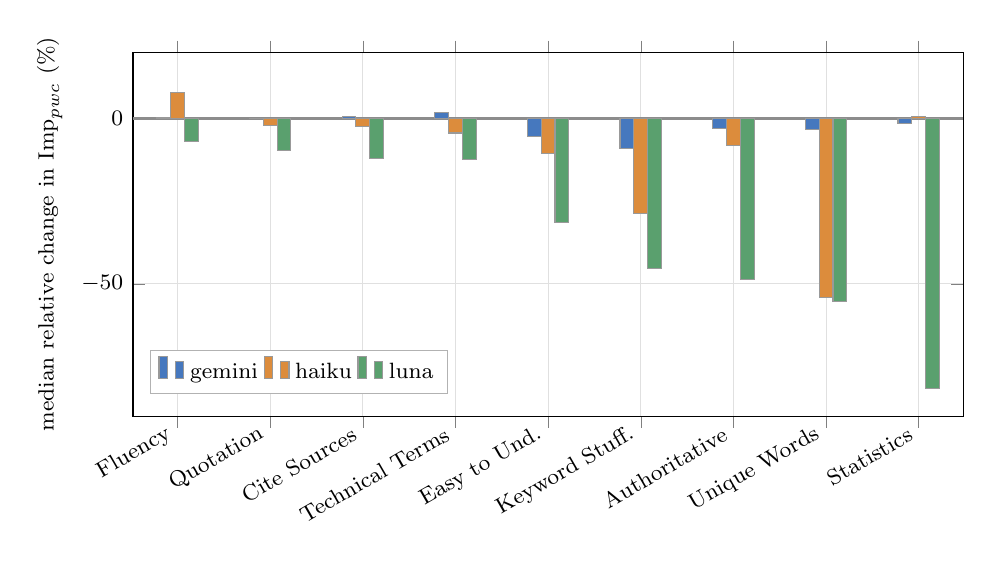
\begin{tikzpicture}
\begin{axis}[
  width=\textwidth, height=6.2cm,
  ybar=0pt, bar width=5pt,
  ymin=-90, ymax=20,
  ylabel={median relative change in $\mathrm{Imp}_{pwc}$ (\%)},
  xtick={0,1,2,3,4,5,6,7,8},
  xticklabels={Fluency,Quotation,Cite Sources,Technical Terms,Easy to Und.,Keyword Stuff.,Authoritative,Unique Words,Statistics},
  x tick label style={rotate=30, anchor=east, font=\footnotesize},
  y tick label style={font=\footnotesize},
  ylabel style={font=\footnotesize},
  legend style={font=\footnotesize, at={(0.02,0.06)}, anchor=south west, draw=black!30},
  legend columns=3,
  grid=major, grid style={black!12},
  enlarge x limits=0.06,
]
\draw[black!45,thick] ({rel axis cs:0,0}|-{axis cs:0,0}) -- ({rel axis cs:1,0}|-{axis cs:0,0});
\addplot[fill=gemblue,draw=black!40] coordinates {(0,0.17) (1,0.01) (2,0.48) (3,1.92) (4,-5.45) (5,-9.10) (6,-3.13) (7,-3.22) (8,-1.45)};
\addlegendentry{gemini}
\addplot[fill=hkorange,draw=black!40] coordinates {(0,7.89) (1,-2.05) (2,-2.33) (3,-4.37) (4,-10.66) (5,-28.62) (6,-8.09) (7,-54.12) (8,0.59)};
\addlegendentry{haiku}
\addplot[fill=lunagreen,draw=black!40] coordinates {(0,-6.89) (1,-9.55) (2,-12.08) (3,-12.41) (4,-31.37) (5,-45.31) (6,-48.68) (7,-55.37) (8,-81.53)};
\addlegendentry{luna}
\end{axis}
\end{tikzpicture}
\caption{Median relative change in target-source visibility per technique, on
each engine, over the primary query set (\texttt{baseline\_pos},
$\mathrm{Imp}_{pwc}$). Techniques are ordered by their worst effect on any
engine. Two things are visible at a glance and are the paper's argument: the
bars are overwhelmingly below zero, and their heights do not agree across
engines --- Statistics Addition is negligible on two engines and $-81.5\%$ on
the third. Exact values, intervals and corrected significance are in
Table~\ref{tab:comparacao_3_engines}.}
\label{fig:efeitos}
\end{figure*}
